\subsection{Chaining blocks}
In the next experiments we experiment with MultiChain creating a chain of blocks between two peers.
The experiments are run using gumby.
In the first experiment we try to create 10 subsequent blocks mimicking a download of 10MB with a speed of 1000 KB/s.
Every second these amounts are indicated to have been transferred to the schedulers of every peer.
The scheduler waits for 1MB uploaded to another peer before scheduling a block.
The result of the experiment can be seen in the graph in Figure \ref{fig:chain-experiment-graph}.
In this graph it can be clearly seen that MultiChain is succesful in creating a chain of 10 blocks.

\begin{figure}[!h]
	\centerline{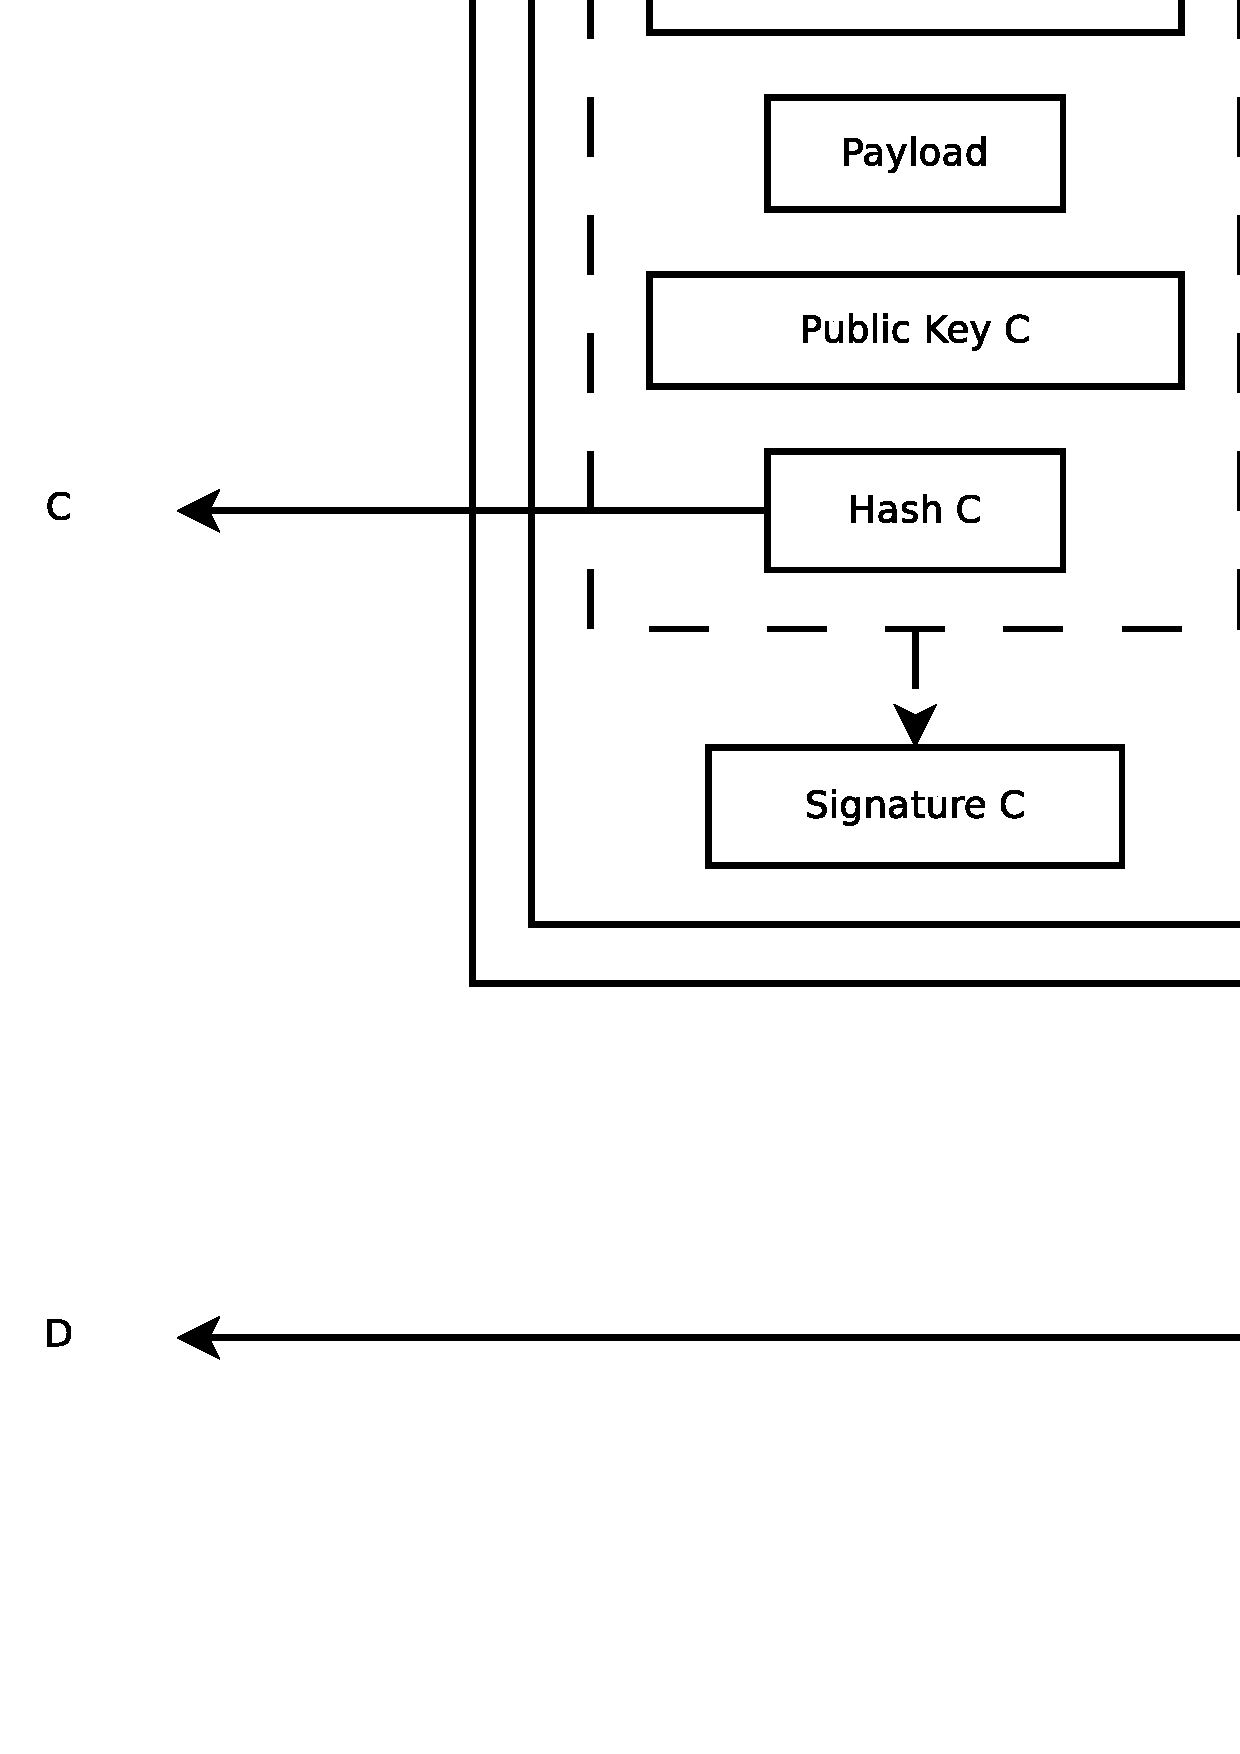
\includegraphics[scale=0.20]{experimentation/chain/chain.png}}
	\caption{MultiChain chain graph of a single download of 10 MB.}
	\label{fig:chain-experiment-graph}
\end{figure}

The amounts stored in each blocks are plotted in Figure \ref{fig:chain-experiment-amounts-small}.
Every datapoint is a block in the chain of a peer and is the the total amount stored in that block..
These datapoints are connected by a dotted line representing the link between these blocks.
These plots show that MultiChain correctly tracks the download of 10MB.
The slope of the figure corresponds with the speed of the download.

\begin{figure}
\centering
\subfigure[Total download amount.]{
\centerline{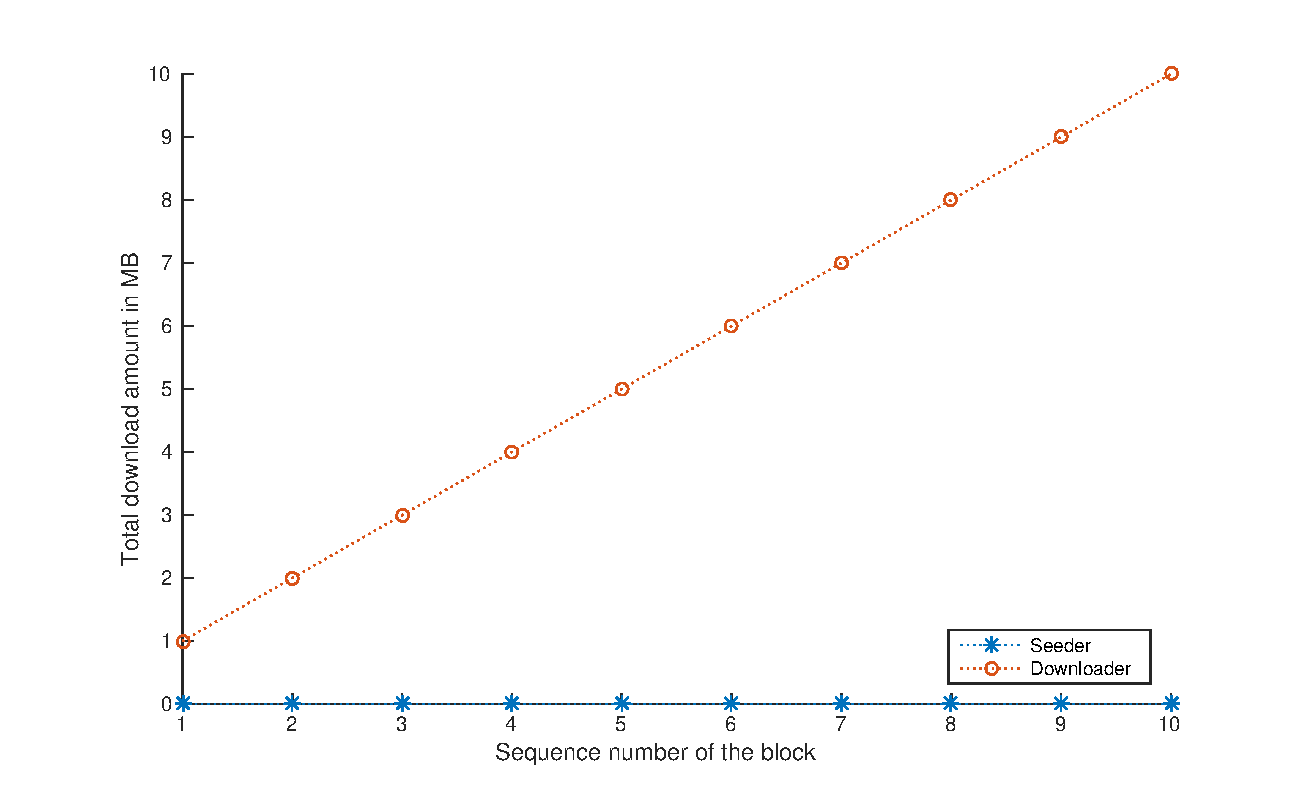
\includegraphics[scale=0.5]{experimentation/chain/small/chain-down.eps}}
\label{fig:chain-experiment-small-down}
}
\subfigure[Total upload amount.]{
\centerline{\includegraphics[scale=0.5]{experimentation/chain/small/chain-up.eps}}
\label{fig:chain-experiment-small-up}
}
\caption{Download and upload amounts when creating a chain of 10 blocks for a 10MB download.}
\label{fig:chain-experiment-amounts-small}
\end{figure}

We also experimented with MutliChain running much longer with a bigger download.
In the following experiment we mimick a download of 10 GB with a speed of 1000 KB/s.
The rest of the setup is the same as in the previous example
and the result is plotted in the same way in Figure \ref{fig:chain-experiment-amounts-long}.
The individual points are obscured by the large amount of points in the figure.
As can be seen in the plots, MultiChain has no problem running for a longer period of time.

\begin{figure}
\centering
\subfigure[Total download amount.]{
\centerline{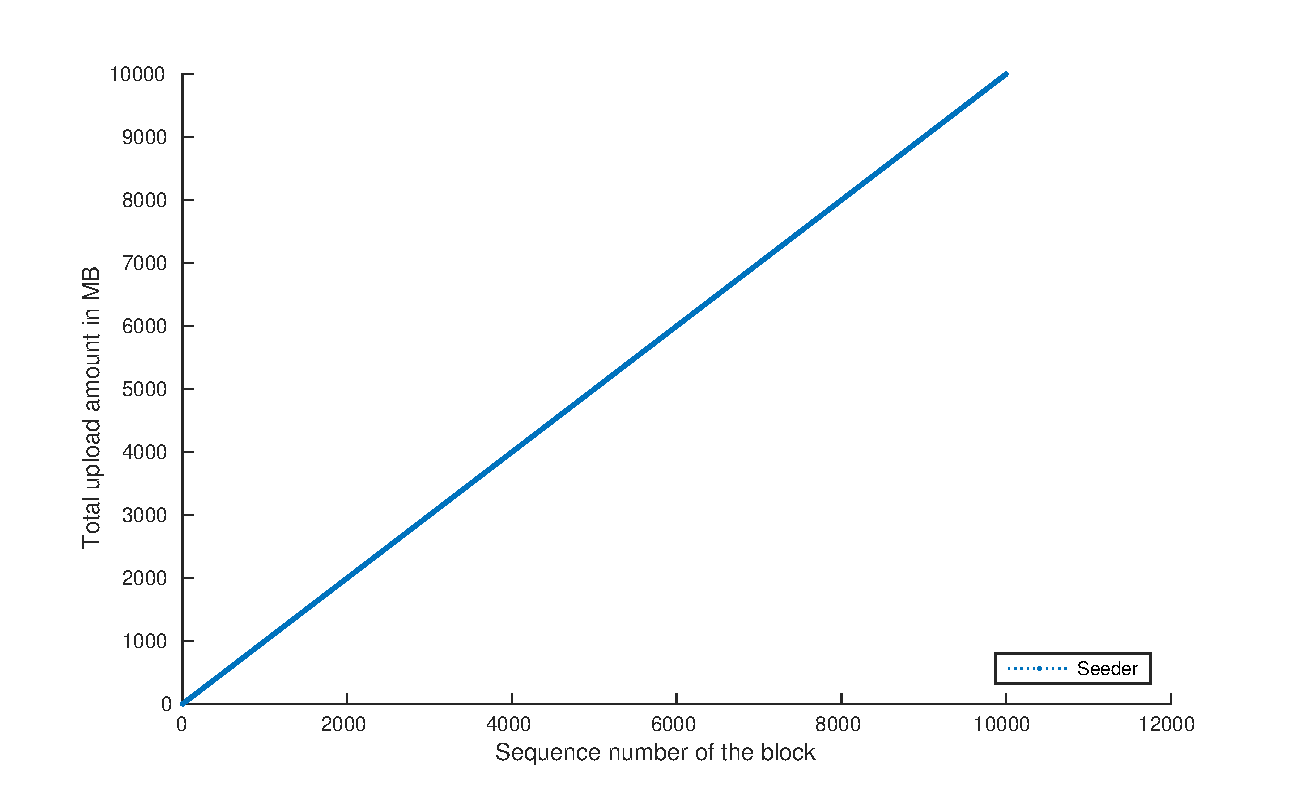
\includegraphics[scale=0.5]{experimentation/chain/long/chain-down.eps}}
\label{fig:chain-experiment-long-down}
}
\subfigure[Total upload amount.]{
\centerline{\includegraphics[scale=0.5]{experimentation/chain/long/chain-up.eps}}
\label{fig:chain-experiment-long-up}
}
\caption{Download and upload amounts when creating a chain of 10 000 blocks for a 10GB download.}
\label{fig:chain-experiment-amounts-long}
\end{figure}